\documentclass[a4paper,11pt]{article}

\usepackage[utf8]{inputenc} % Unicode support (Umlauts etc.)
\usepackage[ngerman]{babel} % Change hyphenation rules
\usepackage{ziffer} % , können in Zahlen verwendet werden ohne Formatierung kaputt zu machen
\usepackage[top=30mm,right=20mm,bottom=15mm,left=25mm,includefoot,headheight=28pt]{geometry} % Seitenränder

\usepackage{lmodern,textcomp} % The package supports the Text Companion fonts, which provide many text symbols (benötigt für €)
\usepackage[fleqn]{amsmath} % Formatierte Gleichungen
\usepackage{graphicx} % Grafiken
\usepackage{xcolor} % Farbe in Text
\usepackage{fancyhdr} % Seitenstil mit Kopfzeile etc.

\pagestyle{fancy}
\fancyhf{}
\lhead{Lösung \\ Übungsblatt 3}
\rhead{Gruppe 8 \\ Michel \textbf{Hansen}, Pascal \textbf{Heinrich}, Nils \textbf{Hodys}, Sascha \textbf{Majewsky}}
\rfoot{Seite \thepage}

\setlength{\parindent}{0cm} % Keine Einrückung der 1. Zeile eines Absatzes

\begin{document}

\raggedright % Alles Linksbündig


\section*{Aufgabe 1}
\subsection*{Ausgangsmodell}
\begin{align*}
\text{max. } & z = 4x_1 - 2x_2 \\
\text{s.t. } & x_3 = 30 - x_1 - 2x_2 \\
& x_4 = {\color{red} -20} - 2x_1 + 2x_2  & \color{red} \to \text{Phase I notwendig} \\
& x_5 = 25 -4x_1 - x_2 \\
& x_1, x_2, x_3, x_4, x_5 \ge 0 \\
\end{align*}

$\to$ Lösung unzulässig, deshalb ist zuerst die Phase I notwendig. \\

\subsection*{Neue Zielfunktion \emph{s}}
\begin{align*}
\text{max. } s &= x_4 \\
&= -20 - 2x1 + {\color{red} 2x_2}
\end{align*}

\begin{align*}
& z = 0 + 4x_1 - 2x_2 \\
& x_3 = 30 - x_1 - 2x_2 &&\big| x_2 \uparrow 15 \\
& x_4 = -20 - 2x_1 + {\color{red} 2x_2} &&\big| \color{red} x_2 \uparrow 10 \\
& x_5 = 25 -4x_1 - x_2 &&\big| x_2 \uparrow 12,5 \\
& x_1, x_2, x_3, x_4, x_5 \ge 0 \\
\end{align*}

\subsection*{Nach Umformen und Einsetzen}
\begin{align*}
\text{max. } & s = x_4 \\
\text{s.t. } & z = -20 + 2x_1 - x_4 \\
& x_2 = 10 + x_1 + \frac{1}{2}x_4 \\
& x_3 = 10 - 3x_1 - x_4 \\
& x_5 = 15 - 5x_1 - \frac{1}{2}x_4 \\
& x_1, x_2, x_3, x_4, x_5 \ge 0
\end{align*}

\subsection*{Simplex Phase II}
\begin{align*}
\text{max. } & z = -20 + {\color{red} 2x_1} - x_4 \\
\text{s.t. } & x_2 = 10 + x_1 + \frac{1}{2}x_4 &&\big| x_1 \le 10 \\
& x_3 = 10 - 3x_1 - x_4 &&\big| x_1 \le \frac{10}{3} \\
& x_5 = 15 - {\color{red} 5x_1} - \frac{1}{2}x_4 &&\big| \color{red} x_1 \le 3 \to \text{minimale Beschränkung} \\
& x_1, x_2, x_3, x_4, x_5 \ge 0
\end{align*}

\subsection*{Nach Umformen und Einsetzen:}
\begin{align*}
\text{max. } & {\color{teal} z = -14} - \frac{2}{10}x_4 - \frac{2}{5}x_5 \\
\text{s.t. } & {\color{teal} x_1 = 3} - \frac{1}{10}x_4 - \frac{1}{5}x_5 \\
& {\color{teal} x_2 = 13} + \frac{2}{5}x_4 - \frac{1}{5}x_5 \\
& x_3 = 1 - \frac{7}{10}x_4 + \frac{6}{5}x_5 \\
& x_1, x_2, x_3, x_4, x_5 \ge 0
\end{align*}

\subsection*{Lösung:}
\begin{align*}
z &= -14 \\
x_1 &= 3 \\
x_2 &= 13
\end{align*}


\section*{Aufgabe 2}
\subsection*{Ausgangsmodell}
\begin{align*}
\text{max. } & z = 5x_1 + x_2 - 2x_3 \\
\text{s.t. } & x_1 + 2x_2 + 3x_3 \le 25 \\
& 5x_1 + 2x_3 = 25 \\
& 3x_1 - 8x_2 \ge 30 \\
& x_1, x_2, x_3 \ge 0
\end{align*}

$\to$ Keine freien Variablen. \\

\subsection*{Gleichungen zu Ungleichungen}
\begin{align*}
\text{max. } & z = 5x_1 + x_2 - 2x_3 \\
\text{s.t. } & x_1 + 2x_2 + 3x_3 \le 25 \\
& 5x_1 + 2x_3 \ge 25 \\
& 5x_1 + 2x_3 \le 25 \\
& 3x_1 - 8x_2 \ge 30 \\
& x_1, x_2, x_3 \ge 0
\end{align*}

$\to$ Bereits eine max-Zielfunktion. \\

\subsection*{Ungleichungen zu Gleichungen mit Schlupfvariablen}
\begin{align*}
\text{max. } & z = 5x_1 + x_2 - 2x_3 \\
\text{s.t. } & x_1 + 2x_2 + 3x_3 + x_4 = 25 \\
& 5x_1 + 2x_3 - x_5 = 25 \\
& 5x_1 + 2x_3 + x_6 = 25 \\
& 3x_1 - 8x_2 - x_7 = 30 \\
& x_1, x_2, x_3, x_4, x_5, x_6, x_7 \ge 0
\end{align*}

\subsection*{Nach BV umgestellt}
\begin{align*}
\text{max. } & z = 5x_1 + x_2 - 2x_3 \\
\text{s.t. } & x_4 = 25 - x_1 - 2x_2 - 3x_3 \\
& {\color{red} x_5 = -25} + 5x_1 + 2x_3 \color{red} \longrightarrow \text{Unzulässig} \\
& x_6 = 25 - 5x_1 - 2x_3 \\
& {\color{red} x_7 = -30} + 3x_1 - 8x_2 \color{red} \longrightarrow \text{Unzulässig} \\
& x_1, x_2, x_3, x_4, x_5, x_6, x_7 \ge 0
\end{align*}

$\to$ Lösung unzulässig, deshalb ist zuerst die Phase I notwendig. \\

\subsection*{Neue Zielfunktion \emph{s}}
\begin{align*}
\text{max. } s &= x_5 + x_7 \\
&= (-25 + 5x_1 + 2x_3) + (-30 + 3x_1 - 8x_2) \\
&= -55 + {\color{red} 8x_1} - 8x_2 + 2x_3
\end{align*}
\begin{align*}
\text{s.t. } & z = 0 + 5x_1 + x_2 - 2x_3 \\
& x_4 = 25 - x_1 - 2x_2 - 3x_3 &&\big| x_1 \uparrow 25 \\
& x_5 = -25 + {\color{red} 5x_1} + 2x_3 &&\big| \color{red} x_1 \uparrow 5 \\
& x_6 = 25 - 5x_1 - 2x_3 &&\big| x_1 \uparrow 5 \\
& x_7 = -30 + 3x_1 - 8x_2 &&\big| x_1 \uparrow 10 \\
& x_1, x_2, x_3, x_4, x_5, x_6, x_7 \ge 0
\end{align*}

\subsection*{Nach Umformen und Einsetzen - Iteration 1}
\begin{align*}
\text{max. } & s = -15 - 8x_2 - \frac{6}{5}x_3 + {\color{red} \frac{8}{5}x_5}\\
\text{s.t. } & z = 25 + x_2 - 4x_3 +x_5 \\
& x_1 = 5 - \frac{2}{5}x_3 + \frac{1}{5}x_5 &&\big| x_5 \uparrow \infty \\
& x_4 = 20 - 2x_2 - \frac{13}{5}x_3 - \frac{1}{5}x_5 &&\big| x_5 \uparrow 100 \\
& x_6 = 0 - {\color{red} x_5} &&\big| \color{red} x_5 \uparrow 0 \\
& x_7 = -15 - 8x_2 - \frac{6}{5}x_3 + \frac{3}{5}x_5 &&\big| x_5 \uparrow 25 \\
& x_1, x_2, x_3, x_4, x_5, x_6, x_7 \ge 0
\end{align*}

\subsection*{Nach Umformen und Einsetzen - Iteration 2}
\begin{align*}
\text{max. } & s = -15 - 8x_2 - \frac{6}{5}x_3 - \frac{8}{5}x_6 \color{red} \longrightarrow \text{Kein positiver Koeffizient mehr} \\
\text{s.t. } & z = 25 + x_2 - 4x_3 +x_5 \\
& x_1 = 5 - \frac{2}{5}x_3 - \frac{1}{5}x_6 \\
& x_4 = 20 - 2x_2 - \frac{13}{5}x_3 + \frac{1}{5}x_6 \\
& x_5 = 0 - x_6 \\
& {\color{red} x_7 = -15} - 8x_2 - \frac{6}{5}x_3 - \frac{3}{5}x_6 \color{red} \longrightarrow \text{Immer noch unzulässig} \\
& x_1, x_2, x_3, x_4, x_5, x_6, x_7 \ge 0
\end{align*}

$\to$ Abbruchbedingung des Simplex-Algorithmus ist erfüllt, es kann keine zulässige Lösung gefunden werden. \\

\vspace{4mm}
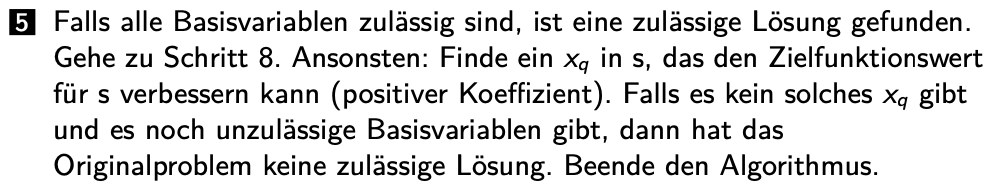
\includegraphics[width=.7\linewidth]{src/unzulaessig.png}

\section*{Aufgabe 3}
\subsection*{a)}
$x_{BA}, x_{HI}, x_{ER}, x_{Row3}, x_{Row6}$, da diese für die Lösung nicht auf 0 gesetzt wurden.

\subsection*{b)}
Die Produktionsmengen bleiben unverändert, da bereits die nach den Restriktionen maximal mögliche Menge Bananeneis produziert wird.

\subsection*{c)}
Ja, es bleiben Zutaten für 7,5 Kugeln / 750g Bananeneis (\emph{Row 3}) über.
Es bleiben Zutaten für 40 Kugeln / 4000g Himbeereis (\emph{Row 6}) über.

\subsection*{d)}
$x_{BA}$ wird bereits maximal produziert.\\
Zulässige Erhöhung: $+ \infty$. \\
Zulässige Reduktion: $-0,1$ € / Kugel. \\

\vspace{4mm}
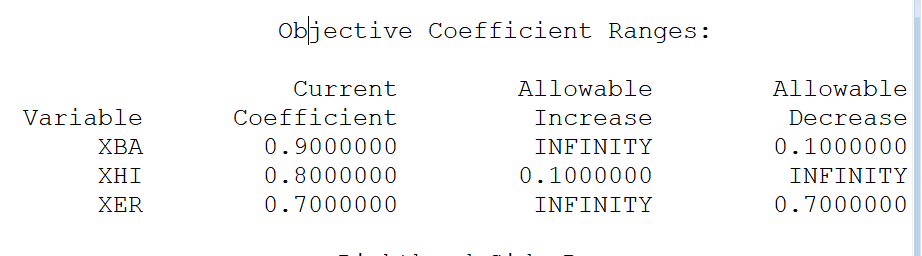
\includegraphics[width=.8\linewidth]{src/zielfunktion.png}

\subsection*{e)}

[Blau] Die Menge der Bananen darf unendlich erhöht werden. Sie darf um die für 7,5 Kugeln notwendige Menge reduziert werden (300g Bananen). \newline

[Grün] Die Menge der Erdbeeren darf nicht erhöht werden. Sie darf um die Menge für 20 Kugeln Eis reduziert werden.

\vspace{4mm}
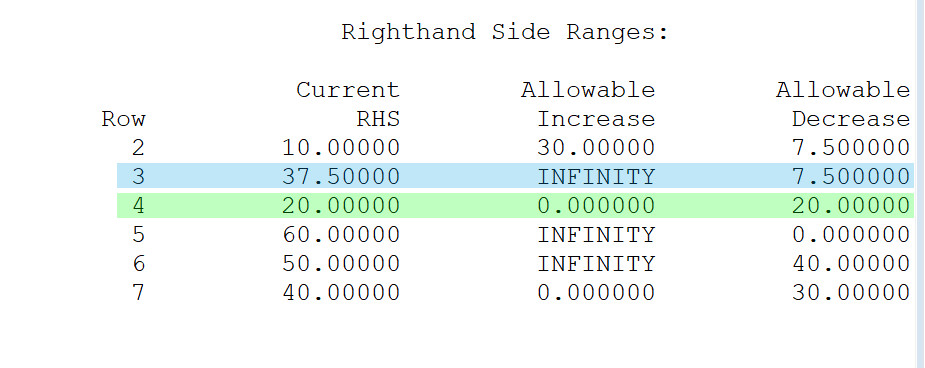
\includegraphics[width=.8\linewidth]{src/restriktionen.png}

\end{document}